\documentclass[a4paper,12pt]{article}
\usepackage[utf8]{inputenc}
\usepackage{cite}
\usepackage{indentfirst}
\usepackage{graphicx}
\usepackage{dblfloatfix}
\usepackage{authblk}
\usepackage{float}

\newcommand*{\Titlefont}{\Large\normalfont}
\renewcommand*{\Authfont}{\normalsize\normalfont}
\renewcommand*{\Affilfont}{\footnotesize\normalfont}

%%%%%%%%%%%%%%%% TABLE
\setlength{\arrayrulewidth}{0.1mm}
\setlength{\tabcolsep}{18pt}
\renewcommand{\arraystretch}{1.5}
\newcommand{\ce}{\centering}

%%%%%%%%%%%%%%%%% HEADING
\title{\Titlefont PHYS CS 15C Research Proposal\\Remotely Operated Vehicle with Visualized Terrain}
\author[1]{\Authfont David Wang}
\author[1]{\Authfont Frank Fu}
\author[1]{\Authfont Yiluo Li}
\affil[1]{\Affilfont College of Creative Studies, University of California, Santa Barbara}

\begin{document}

\maketitle

\section{Introduction}
Often times there exist terrain on which people cannot tread on. Imagine the complex structure of the debris after an earthquake or hurricane, where an external force of a human footstep might cause additional collapse of the structure, putting victims under it in further danger. However, we would still like to conduct massive search for survivors under the debris. General search could be done by some high-end device far away, and close up confirmation for each potential signal of life could be carried out by smaller sized vehicles such as drones and ground robots. While drones have high mobility around, the ground robot can go under debris to get closer to the survivors. By carrying necessary communication tools and sensors, we could get specific conditions of the survivors, which would be immensely helpful in forming the rescue plan accordingly.
%%%%%%%%%%%%%
\\\indent However, even when a signal of life has been detected, there are still obstacles. Removing the top layers of debris might do damage to the lower layer. Depending on the actual situation of the victim and the structure above the victim, a mature rescue plan might take hours to be finalized. Time is an important factor in this process. To earn more time and make sure the victim can stay with us, a ground robot that have access to the victim could then provide necessary care such as food, water, conversation, and hope to stabilize the conditions of the victim.
%%%%%%%%%%%%%
\\\indent In this project, we propose to control the robot with a visualized terrain that serves like a sandbox in military planning. This visualized terrain inspired by project Electrick \cite{Zhang2017} will provide visual aid to help anyone just arriving grasp the overall picture and the current progress of the rescue plan. Viewer should be able to identify all the potential, confirmed, and successfully saved signals of life as well as the location of the robots and their past and queued trajectories and missions.


\section{Significance}

Traditionally, to manipulate a robot, a person needs to be trained specifically to master its control before actually being proficient enough to conduct the task. However, even so the commander of the task is usually not the direct person to manipulate the robots and his/her command can be delayed when delivering to a certain personal. In this process of commanding, it is possible that a mis-communication happens and leads to fatal failures.

Controlling a robot with a visualized terrain does not merely keep all the personals in the commanding room aware of the most recent update of the situation, but it also saves time for delivering commands and avoid misunderstanding. To control the robot, the decision maker just need to use his/her finger or any conductive baton to draw a path on the visualized terrain. Then, the signals from the terrain will be sent to inform the robot of the path. 

Therefore, this visualized terrain will provide us with more efficiency and accuracy for the rescue mission. In addition, the decision maker can deliver the commands to the robot immediately upon finalization on path planning.

\section{Objective}

\begin{enumerate}
	\item Construct the conductive control pad that serves as the visualized terrain model;
	\item Read in path planned by touch control on the terrain model; 
	\item Build the self-balancing robot with wireless receiver module;
	\item Move the robot according the path planned on the terrain model.
\end{enumerate}


\section{Methodology}
\indent We will first assemble the conductive layer control pad and mound on the electrodes. The conductive layer can be made from coding a square sheet  with carbon conductive paint. Two thin copper chips will be soldered to each side of the control pad to achieve minimum requirement for visualizing the current density map. To supply current, we will use alligator clips jumper wires for easy transfers between different control pads. Each wire that is connected to the control pad will be divided into two, and will be connected to separate voltage source and analog input pins on the Arduino Mega 2560. The chip does not have large enough internal resistance, but as we are merely concerned with where the voltage drop occurs, this error, although large, does not affect the performance of constructing the current density map.
%%%%%%%%%%
\\\indent To construct the current density map, we will supply current through one pair of electrode, and measure the voltage at other vertices connected by two electrodes. Doing the same process repeatedly, we will obtain a mesh of cross sectional measurement as seen in \textbf{Figure \ref{fig:electrick}}, and from this web, we can visualize the current density map to identify the point of contact.


\begin{figure}[t]
	\centering
	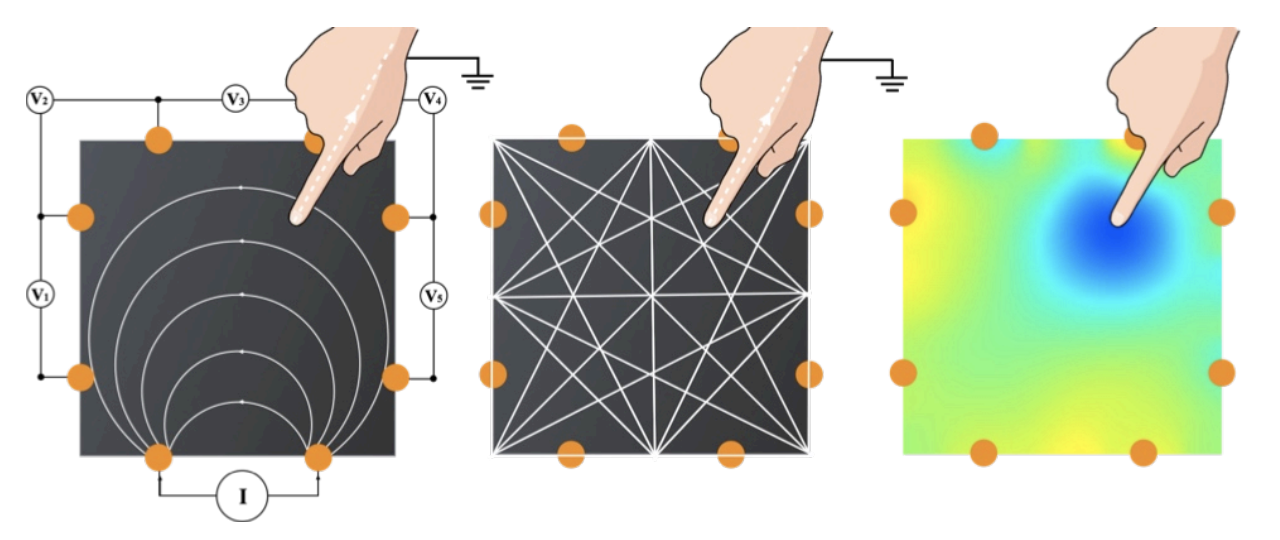
\includegraphics[width=5in]{graph.png}
	\caption{Left: Current is provided in one pair of electrodes and voltage of all other electrodes are measured. Center: a mesh of cross sectional measurements. Right: A processed 2D graph showing current density. Blue color has the lowest current density, indicating location of finger.\cite{Zhang2017}}
	\label{fig:electrick}
\end{figure}

\indent After the control pad works properly, we will work on building the robot. We will use the NCR 18650 battery as power source, GY-521 module as accelerometer, and Arduino Pro Mini for controlling the self-balancing robot. To prevent jamming of wheels in some situations, we would also use ABS breaking system. The DRV 8833 motor driver can provide 1.2 A of current continuously, so this should provide the robot enough power to travel through different terrains. We would write a negative feedback program to use the accelerometer and gyroscope for the robot to balance first, and then maneuver it on flat surfaces. Ideally, we could then modify the program so the robot can travel through all terrains. The signals will be sent wirelessly using the Arduino HC-05 bluetooth module. And the robot should respond promptly after upon receiving the instructions.


\section{Proposed Project Timeline}

$$
\begin{tabular}{ |p{1cm}|p{10cm}|  }
	\hline
		\multicolumn{2}{|c|}{Research Timeline} \\
	\hline
		 Week & Description \\
	\hline
		\ce 1		& 	Order necessary parts\\
		\ce 2		&	Assemble the conductive layer control pad, supply constant AC current through one pair of electrodes, and measure the voltage difference at different vertices\\
		\ce 3-4		&	Supply current through all adjacent pairs of electrodes, and readout the voltage differences at all other vertices\\
		\ce 5-6		&	Visualize the 2-D voltage current density	when touching the control pad with tomography imaging\\
		\ce 7		&	Output coordinate of touch on the control pad; assemble the self-balancing robot\\
		\ce 8-9		&	Assemble the self-balancing robot and the bluetooth module\\
		\ce 10		&	Move the robot with control pad\\
	\hline
\end{tabular}
$$


\section{Budget}
$$
\begin{tabular}{ |p{8cm}|p{1.3cm}|p{1.3cm}|  }
	\hline
		\multicolumn{3}{|c|}{Budget Planning} \\
	\hline
		 Item & Amount & Price(\$) \\
	\hline
		 6" x 6" copper sheet									& 	1	&	7.00\\
		 Jumper with aligator clips								&	20	&	15.98\\
		 Jumper	pack												&	1	&	6.98\\
		 ABS by Zen Tool Works								&	1	&	46.00\\
		 Carbon conductive paint by MG Chemicals	&	2	&	32.00\\
		 Arduino Mega												&	1	&	33.49\\
		 Arduino Pro Mini											&	1	&	9.95\\
		 FTDI friend													&	1	&	14.75\\
		 GY-521 module with MPU-6050					&	1	&	5.99\\
		 DRV8833 Pololu motor driver						&	1	&	4.95\\
		 5V boost converter										&	2	&	1.78\\
		 NCR18650 battery and holder						&	1	&	3.06\\
		 Micro metal gear motors and brackets			&	2	&	11.42\\
		 42 x 19 mm wheels										&	2	&	2.90\\
		 Double-sided prototype PCB pack				&	1	&	6.57\\
		 25 cm Nylon spacers pack							&	2	&	4.38\\
		 Nylon nuts pack											&	1	&	1.15\\
		 Estimated shipping and tax							&	/	&	50\\
		 Misc. modules												& /	& 	50\\
	\hline
		\multicolumn{2}{|c|}{Grand Total}	& 308.35\\
	\hline
\end{tabular}
$$

\section{Conclusion}
\indent The rescue process is often complicated for survivors in debris left by a natural disaster such as earthquake and hurricane. In order to save time and stabilize the survivors, we propose this remotely operated ground robot with visualized terrain that can serve as visual aid in planning the process and communicating the rescue end directly with the survivor end.

%\section{Acknowledgment}


\medskip

%%%%%%%%%%%%%%%%%%%%%%%%%%%%%%%%%%%%%%% CITATION
\bibliographystyle{phaip}
\bibliography{ref}

\end{document}
